\documentclass[fleqn]{article}
\oddsidemargin 0.0in
\textwidth 6.0in
\thispagestyle{empty}
\usepackage{import}
\usepackage{amsmath}
\usepackage{graphicx}
\usepackage{flexisym}
\usepackage{calligra}
\usepackage{amssymb}
\usepackage{bigints} 
\usepackage[english]{babel}
\usepackage[utf8x]{inputenc}
\usepackage{float}
\usepackage[colorinlistoftodos]{todonotes}


\DeclareMathAlphabet{\mathcalligra}{T1}{calligra}{m}{n}
\DeclareFontShape{T1}{calligra}{m}{n}{<->s*[2.2]callig15}{}
\newcommand{\scriptr}{\mathcalligra{r}\,}
\newcommand{\boldscriptr}{\pmb{\mathcalligra{r}}\,}

\definecolor{hwColor}{HTML}{442020}

\begin{document}

  \begin{titlepage}

    \newcommand{\HRule}{\rule{\linewidth}{0.5mm}}

    \center

    \begin{center}
      
\includegraphics[height=11cm, width=11cm]{asu.png}
    \end{center}

    \vline

    \textsc{\LARGE Classical Parts/Field/Matter III}\\[1.5cm]

    \HRule \\[0.5cm]
    { \huge \bfseries Homework Three}\\[0.4cm] 
    \HRule \\[1.0cm]

    \textbf{Behnam Amiri}

    \bigbreak

    \textbf{Prof: Samuel Teitelbaum}

    \bigbreak

    \textbf{{\large \today}\\[2cm]}

    \vfill

  \end{titlepage}

  \begin{enumerate}
    \item \textbf{9.8 (30 points)} Equation $9.36$ describes the most general \textbf{linearly} polarized wave on a string. 
    Linear (or “plane”) polarization (so called because the displacement is parallel to a fixed vector $\hat{n}$) results
    from the combination of horizontally and vertically polarized waves of the \emph{same phase} (Eq. $9.39$). If the two 
    components are of equal amplitude, but out of phase by $90^{\circ}$ (say, $\delta_v=0$, $\delta_h=90^{\circ}$), the result is a circularly
    polarized wave. In that case:
    \begin{enumerate}
      \item At a fixed point $z$, show that the string moves in a circle about the $z$ axis. Does it go \emph{clockwise} or 
      \emph{counterclockwise}, as you look down the axis toward the origin? How would you construct a wave circling the 
      other way? (In optics, the clockwise case is called \textbf{right circular polarization}, and the counterclockwise, \textbf{left
      circular polarization}.)
      \\
      \emph{An elegant notation for circular polarization (or elliptical, if the amplitudes are unequal) is to use a
      complex $\hat{n}$, but I shall not do so in this book.}

        \textcolor{hwColor}{
          \\
          Equation $9.36$ and $9.39$ from the textbook are
          \\
          \\ 
          $
            \tilde{f}(z,t)=\tilde{A} ~ e^{i(kz-\omega t)} ~ \hat{n} ~~~~~~~~~~~~~~~~~~~~~~~~~~~~~~~~~~~~~~~~~~~~~~~~ (9.36)
            \\
            \\
            \tilde{f}(z,t)=\left(\tilde{A} ~ cos(\theta)\right) e^{i(kz-\omega t)} \hat{x}
            +\left(\tilde{A} ~ sin(\theta)\right) e^{i(kz-\omega t)} \hat{y} ~~~~~ (9.39)
            \\
            \\
          $
          Electromagnetic waves are transverse. There are two dimensions perpendicular to any given line of propagation. Transverse waves
          occur in two independent states of polarization. If the two components are of equal amplitude, but out of phase by $90^{\circ}$
          , the result is circularly polarized wave. Then
          $
            \\
            \\
            \tilde{f}(z,t)=A ~ e^{i(kz-\omega t)} ~ \hat{x}+A ~ e^{i(kz-\omega t+\dfrac{\pi}{2})} ~ \hat{y}
            =A \left[\hat{x}+e^{i \dfrac{\pi}{2}} ~ \hat{y}\right] ~ e^{i(kz-\omega t)}
            \\
            \\
            \\
            \therefore ~~~ \boxed{\tilde{f}(z,t)=A \left(\hat{x}+i ~ \hat{y}\right) e^{i(kz-\omega t)}} ~~~~ \checkmark
          $
          \\
          \\
          For simplicity, let's $z=0$ so we have
          \\
          \\
          $
            \tilde{f}(0,t)=A \left(\hat{x}+i ~ \hat{y}\right) e^{-i\omega t}
            =A \left(\hat{x}+i ~ \hat{y}\right) \times \left[cos(\omega t)+i ~ sin(-\omega t)\right]
            \\
            \\
            =A \left(\hat{x}+i ~ \hat{y}\right) \times \left[cos(\omega t)-i ~ sin(\omega t)\right]
            =A \left[
              cos(\omega t) ~ \hat{x}
              -i ~ sin(\omega t) ~ \hat{x}
              +i ~ cos(\omega t) ~ \hat{y}
              -i ~ i ~ sin(\omega t) ~ \hat{y}
            \right]
            \\
            \\
            =Re\left[A \left(
              cos(\omega t)~ \hat{x}+sin(\omega t) ~ \hat{y}
            \right)\right]
          $
          \\
          \\
          In above we assume that $A$ is real and the real part of these equations are what we are interested in.
          \\
          \\
          \\
          $
            \therefore ~~~ \boxed{
              \begin{cases}
                \text{X-direction}: ~ f=cos(\omega t)~ \hat{x}
                \\
                \\
                \text{Y-direction}: ~ f=sin(\omega t) ~ \hat{y}
              \end{cases}
            } ~~~~ \checkmark
            \\
          $
          \\
          \\
          We are familiar with this equation back from \textbf{Calculus} which is nothing but the equation of a circle. This circle goes 
          counter-clockwise as we look down the axis toward the origin. 
          \\
          \\
          In order to construct a wave circling the other way, all we need to do is switching the sign of phase difference between the two
          $(-90^{\circ})$.
          \\
          \\
        }

      \item Sketch the string at time $t = 0$.

        \begin{figure}[h!]
          \centering
          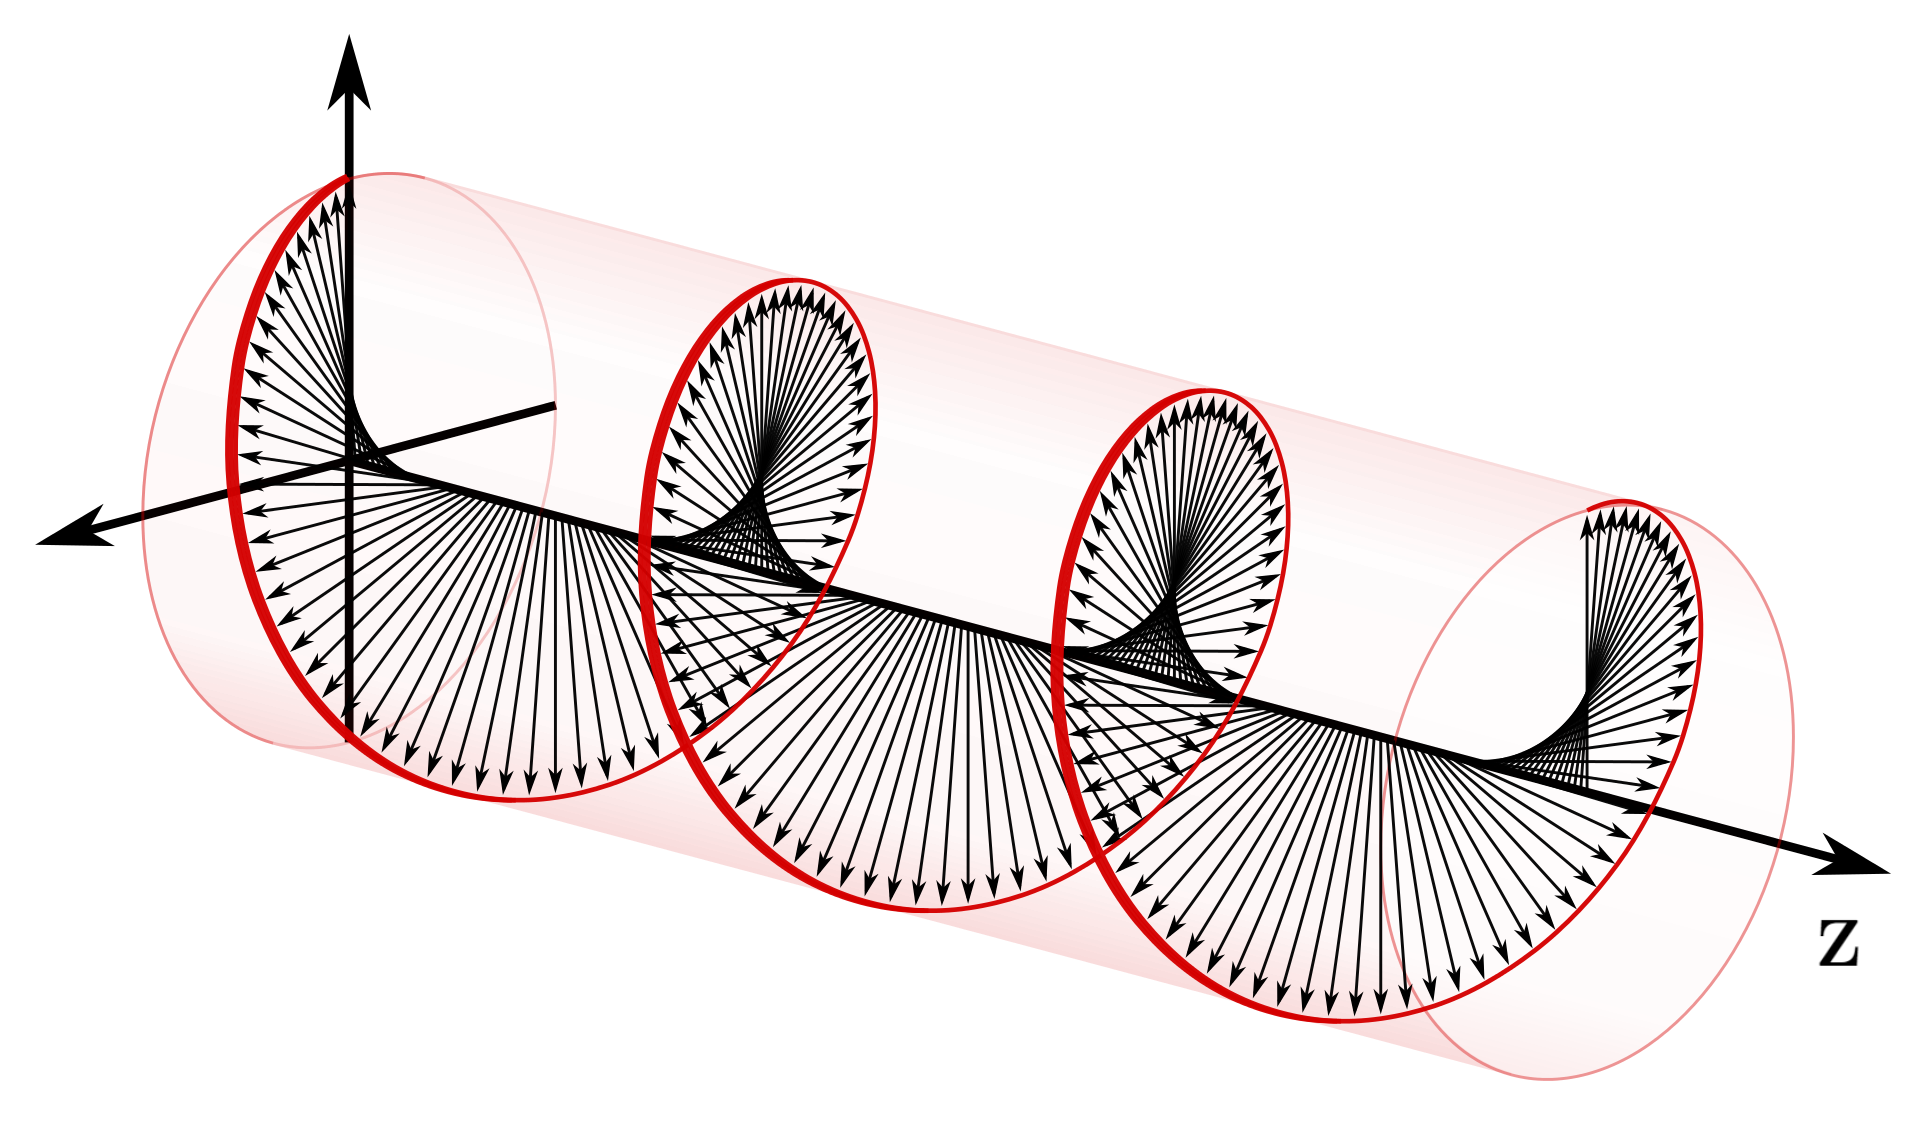
\includegraphics[height=7cm, width=12cm]{1.png}
          \caption{
            This figure is taken from Wikipedia. 
          }
        \end{figure}


      \item How would you shake the string in order to produce a circularly polarized wave?
      
        \textcolor{hwColor}{
          \\
          To answer this question we can picture battle ropes at the gym. In order to produce a circularly polarized waved with them, all we
          need to do is rotating our arms in circle.
          \\
        }

    \end{enumerate}

    \pagebreak

    \item \textbf{9.13 (40 points)} Find all elements of the Maxwell stress tensor for a monochromatic plane wave traveling in the 
    $z$ direction and linearly polarized in the $x$ direction (Eq. $9.48$). Does your answer make sense? (Remember that 
    $-\overleftrightarrow{T}$ represents the momentum flux density.) How is the momentum flux density related to the energy
    density, in this case?

      \textcolor{hwColor}{
        \\
        Equation $9.48$ from the textbook
        \\
        \\
        $
          \begin{cases}
            E(z,t)=E_0 ~ cos(kz-\omega t+\delta) ~ \hat{x}
            \\
            \\
            B(z,t)=\dfrac{1}{c} E_0 ~ cos(kz-\omega t+\delta) ~ \hat{y}
          \end{cases}
        $
        \\
        \\
      }
      \begin{center}
        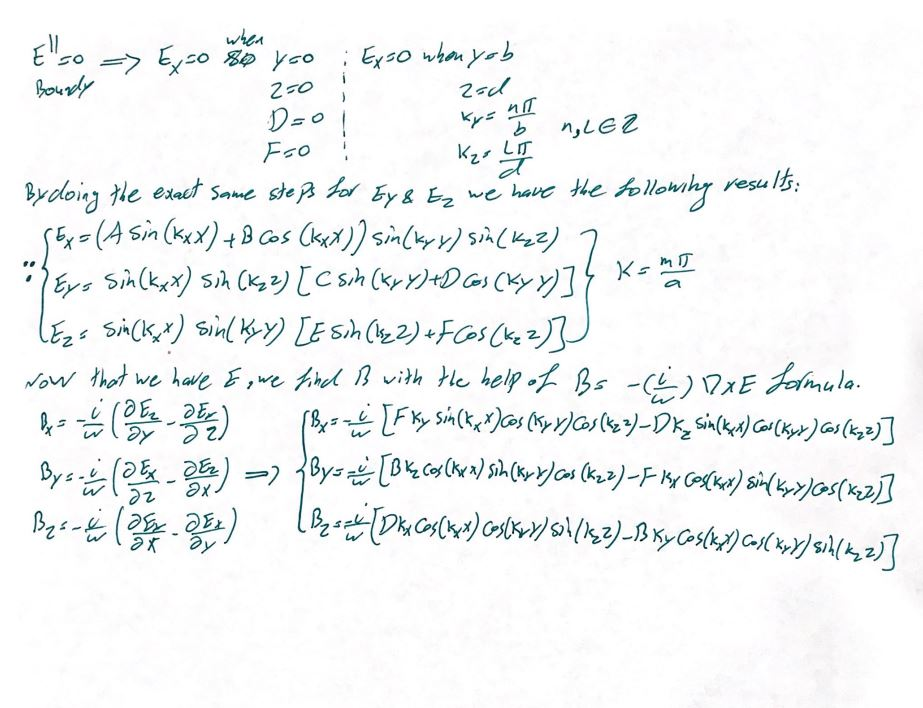
\includegraphics[height=5cm, width=12cm]{2.JPG}
      \end{center}
      \textcolor{hwColor}{    
        \\
        \\
        In chapter 8, we learned about the \textbf{Maxwell stress tensor}. Let's rewrite again here. Note the  \textbf{Kronecker delta},
        $\delta_{ij}$ is $1$ if the indices are the same $(\delta_{xx}=\delta_{yy}=\delta_{zz}=1)$ and zero otherwise
        $(\delta_{xy}=\delta_{xz}=\delta_{yz}=0)$. Also, $c^2=\dfrac{1}{\mu_0 ~ \epsilon_0}$ comes from the wave equation that  
        can be derived from Maxwell's equations.
        \\
        \\
        $
          T_{ij} \equiv \epsilon_0 \left(E_i ~ E_j -\dfrac{1}{2} \delta_{ij} ~ E^2 \right)
          +\dfrac{1}{\mu_0} \left(B_i ~ B_j -\dfrac{1}{2} \delta_{ij} B^2 \right) ~~~~~~~~~~~~~~~ (8.17)
          \\
          \\
          \\
          \overleftrightarrow{T}=\begin{pmatrix}
            T_{xx} & T_{xy} & T_{xz} 
            \\
            T_{yx} & T_{yy} & T_{yz} 
            \\
            T_{zx} & T_{zy} & T_{zz} 
          \end{pmatrix}
          \\
          \\
          \\
          T_{xx}=\epsilon_0 \left(E_x ~ E_x -\dfrac{1}{2} \delta_{xx} ~ E^2 \right)
          +\dfrac{1}{\mu_0} \left(B_x ~ B_x -\dfrac{1}{2} \delta_{xx} B^2 \right)
          \\
          =\epsilon_0 \left(E_0 ~ E_0 -\dfrac{1}{2} ~ E_0^2 \right)
          +\dfrac{1}{\mu_0} \left(0 -\dfrac{1}{2} \left(\dfrac{1}{c} E_0\right)^2 \right)
          =\epsilon_0 \left(E_0^2 -\dfrac{1}{2} ~ E_0^2 \right)
          +\dfrac{1}{\mu_0} \left(-\dfrac{1}{2c^2} E_0^2 \right)
          \\
          =\dfrac{1}{2} \left[
            \epsilon_0 ~ E_0^2
            -\dfrac{1}{\mu_0 c^2} E_0^2
          \right]
          =\dfrac{1}{2} \left[
            \epsilon_0 ~ E_0^2
            -\epsilon_0 E_0^2
          \right]       
          \\
          \\
          \\
          \therefore ~~~ \boxed{T_{xx}=0} ~~~~ \checkmark
          \\
          \\
          \\
          \\
          T_{xy}=\epsilon_0 \left(E_x ~ E_y -\dfrac{1}{2} \delta_{xy} ~ E^2 \right)
          +\dfrac{1}{\mu_0} \left(B_x ~ B_y -\dfrac{1}{2} \delta_{xy} B^2 \right)
          \\
          =\epsilon_0 \left(E_0 \times 0 -\dfrac{1}{2} \times 0 \times ~ E_0^2 \right)
          +\dfrac{1}{\mu_0} \left(0 \times \dfrac{1}{c}E_0 -\dfrac{1}{2} \times 0 \times \left(\dfrac{1}{c}E_0\right)^2 \right)
          \\
          \\
          \\
          \therefore ~~~ \boxed{T_{xy}=0} ~~~~ \checkmark
          \\
          \\
          \\
          \\
          T_{xz}=\epsilon_0 \left(E_x ~ E_z -\dfrac{1}{2} \delta_{xz} ~ E^2 \right)
          +\dfrac{1}{\mu_0} \left(B_x ~ B_z -\dfrac{1}{2} \delta_{xz} B^2 \right)
          \\
          =\epsilon_0 \left(E_0 \times 0 -\dfrac{1}{2} \times 0 \times E_0^2 \right)
          +\dfrac{1}{\mu_0} \left(0 \times 0 -\dfrac{1}{2} \times 0 \times \left(\dfrac{1}{c}E_0\right)^2 \right)
          \\
          \\
          \\
          \therefore ~~~ \boxed{T_{xz}=0} ~~~~ \checkmark
          \\
          \\
          \\
          \\
          T_{yx}=\epsilon_0 \left(E_y ~ E_x -\dfrac{1}{2} \delta_{yx} ~ E^2 \right)
          +\dfrac{1}{\mu_0} \left(B_y ~ B_x -\dfrac{1}{2} \delta_{yx} B^2 \right)
          \\
          =\epsilon_0 \left(0 \times E_0 -\dfrac{1}{2} \times 0 \times ~ E_0^2 \right)
          +\dfrac{1}{\mu_0} \left(\dfrac{1}{c}E_0 \times 0 -\dfrac{1}{2} \times 0 \times \left(\dfrac{1}{c}E_0\right)^2 \right)
          \\
          \\
          \\
          \therefore ~~~ \boxed{T_{yx}=0} ~~~~ \checkmark
          \\
          \\
          \\
          \\
          T_{yy}=\epsilon_0 \left(E_y ~ E_y -\dfrac{1}{2} \delta_{yy} ~ E^2 \right)
          +\dfrac{1}{\mu_0} \left(B_y ~ B_y -\dfrac{1}{2} \delta_{yy} B^2 \right)
          \\
          =\epsilon_0 \left(0 \times 0 -\dfrac{1}{2} ~ E_0^2 \right)
          +\dfrac{1}{\mu_0} \left(\left(\dfrac{1}{c}E_0\right)^2 -\dfrac{1}{2} \left(\dfrac{1}{c}E_0\right)^2 \right)
          \\
          =-\dfrac{1}{2} \epsilon_0 ~ E_0^2+\dfrac{1}{\mu_0} \dfrac{1}{2} \dfrac{E_0^2}{c^2}
          \\
          \\
          \\
          \therefore ~~~ \boxed{T_{yy}=0} ~~~~ \checkmark
          \\
          \\
          \\
          T_{yz}=\epsilon_0 \left(E_y ~ E_z -\dfrac{1}{2} \delta_{yz} ~ E^2 \right)
          +\dfrac{1}{\mu_0} \left(B_y ~ B_z -\dfrac{1}{2} \delta_{yz} B^2 \right)
          \\
          =\epsilon_0 \left(0 \times 0 -\dfrac{1}{2} \times 0 \times ~ E_0^2 \right)
          +\dfrac{1}{\mu_0} \left(\dfrac{1}{c}E_0 \times 0 -\dfrac{1}{2} \times 0 \times \left(\dfrac{1}{c}E_0\right)^2 \right)
          \\
          \\
          \\
          \therefore ~~~ \boxed{T_{yz}=0} ~~~~ \checkmark
          \\
          \\
          \\
          \\
          T_{zx}=\epsilon_0 \left(E_z ~ E_x -\dfrac{1}{2} \delta_{zx} ~ E^2 \right)
          +\dfrac{1}{\mu_0} \left(B_z ~ B_x -\dfrac{1}{2} \delta_{zx} B^2 \right)
          \\
          =\epsilon_0 \left(0 \times E_0 -\dfrac{1}{2} \times 0 \times ~ E_0^2 \right)
          +\dfrac{1}{\mu_0} \left(0 \times 0 -\dfrac{1}{2} \times 0 \times \left(\dfrac{1}{c}E_0\right)^2 \right)
          \\
          \\
          \\
          \therefore ~~~ \boxed{T_{zx}=0} ~~~~ \checkmark
          \\
          \\
          \\
          \\
          T_{zy}=\epsilon_0 \left(E_z ~ E_y -\dfrac{1}{2} \delta_{zy} ~ E^2 \right)
          +\dfrac{1}{\mu_0} \left(B_z ~ B_y -\dfrac{1}{2} \delta_{zy} B^2 \right)
          \\
          =\epsilon_0 \left(0 \times 0 -\dfrac{1}{2} \times 0 \times ~ E_0^2 \right)
          +\dfrac{1}{\mu_0} \left(0 \times \dfrac{1}{c}E_0 -\dfrac{1}{2} \times 0 \times \left(\dfrac{1}{c}E_0\right)^2 \right)
          \\
          \\
          \\
          \therefore ~~~ \boxed{T_{zy}=0} ~~~~ \checkmark
          \\
          \\
          \\
          \\
          T_{zz}=\epsilon_0 \left(E_z ~ E_z -\dfrac{1}{2} \delta_{zz} ~ E^2 \right)
          +\dfrac{1}{\mu_0} \left(B_z ~ B_z -\dfrac{1}{2} \delta_{zz} B^2 \right)
          \\
          =\epsilon_0 \left(0 \times 0 -\dfrac{1}{2} ~ \left(E_0 ~ cos(kz-\omega t+\delta)\right)^2 \right)
          +\dfrac{1}{\mu_0} \left(0 \times 0 -\dfrac{1}{2} \left(\dfrac{1}{c} E_0 ~ cos(kz-\omega t+\delta) \right)^2 \right)
          \\
          =-\dfrac{1}{2} \epsilon_0 ~ E_0^2 ~ cos^2(kz-\omega t+\delta)-\dfrac{1}{2} \dfrac{1}{\mu_0 ~ c^2} E_0^2 ~ cos^2(kz-\omega t+\delta)
          \\
          =-\dfrac{1}{2} ~ \epsilon_0 ~ E_0^2 ~ cos^2(kz-\omega t+\delta)-\dfrac{1}{2} ~ \epsilon_0 ~ E_0^2 ~ cos^2(kz-\omega t+\delta)
          \\
          \\
          \\
          \therefore ~~~ \boxed{T_{zz}=-\epsilon_0 ~ E_0^2 ~ cos^2(kz-\omega t+\delta)} ~~~~ \checkmark
          \\
          \\
        $
        All elements of the Maxwell stress tensor vanished except $T_{zz}$. Well, this justifies that the momentum of the fields points in the
        Z-direction which makes sense. Also, we know that $E_0^2 ~ cos^2(kz-\omega t+\delta)=-T_{zz}$ is the momentum flux density
        \\
        The stress tensor can be considered as \emph{momentum flux density} tensor
      }


    \item \textbf{9.14 (30 points)} Calculate the exact reflection and transmission coefficients, without assuming $\mu_1=\mu_2=\mu_0$. 
    Confirm that $R+T=1$.

      % \textcolor{hwColor}{
      %   \\
      % }


    \item \textbf{9.7 (10 points)} Suppose string $2$ is embedded in a viscous medium (such as molasses), which imposes a drag force 
    that is proportional to its (transverse) speed:
    $$
      \Delta F_{drag}=-\gamma \dfrac{\partial f}{\partial t} ~ \Delta z
    $$
    \begin{enumerate}
      \item Derive the modified wave equation describing the motion of the string.

        % \textcolor{hwColor}{
        %   \\
        % }

      \item Solve this equation, assuming the string vibrates at the incident frequency $\omega$. That is, look for solutions of the
      form $\tilde{f}(z,t)=e^{i \omega t} ~ \tilde{F}(z)$.

        % \textcolor{hwColor}{
        %   \\
        % }

      \item Show that the waves are \textbf{attenuated} (that is, their amplitude decreases with increasing $z$). Find the characteristic penetration distance, at which the amplitude
      is $1/e$ of its original value, in terms of $\gamma$ , $T$, $\mu$, and $\omega$.

        % \textcolor{hwColor}{
        %   \\
        % }

      \item If a wave of amplitude $A_I$ , phase $\delta_I=0$, and frequency $\omega$ is incident from the left (string 1), find the reflected wave’s
      amplitude and phase.

        % \textcolor{hwColor}{
        %   \\
        % }

    \end{enumerate}


  \end{enumerate}

\end{document}
